\chapter{Results and Discussion}


\section{Piezo1 as integrator of biomechanical events}

Piezo1 has been established as important mechanosensation integrator\cite{Murthy2017PiezosTU} \myworries{Two Papers from Mendeley} in a plethora of different physiological contexts. Here we address the issue of transferability and want to find out, whether Piezo1 is equally important in the mechanosensing by mesenchymal stem cells.

Making use of in-house developed Flowchambers and a straightforward calcium imaging protocol, we measured an increase of maximal relative fluorescence levels directly relating to shear stress. Follow up experiments, with knock-out cell lines, indicated that Piezo1 is the main trigger, as calcium-response was lacking in  Piezo1 KO Cell lines.


\subsection{Functionalization of Medium}
To eleminate ER-release of intracellularly stored Ca2+ ions as an explanation for the shear-related effect before \myworries{suggestive!}, we designed an experiment, with the medium as the experimental condition. Flushing the same flowchamber twice, one time with calcium-free ACSF and another time with normal ACSF, we saw an average of 40\% increase in measured $F_{max}/F_{0}$ levels ($n=3$ biological replicates).\par
To conclude, this result combined with the results from before shows that not only do MSC also feel shear stress, but the associated extracellular calcium ion influx is \Piezo mediated. 


\section{Piezo and the extracellular matrix}

Preliminary mass spectroscopy secretome analysis of \Yoda-treated cells showed a distinct decrease in core extracellular matrix (ECM) components, such as alpha-1 type I collagen(\colone), \myworries{Fibronectin-1 (\textsc{Fn1})} and finally alpha-1 type III collagen (\colthree), when compared to control.
This inspired further investigation into this matter.

We set the experiment up, such that we could measure Protein and RNA content from the identical sample to cross-validate our results.  

We extracted the cell By measures of SDS-PAGE, we were able to compare intracellular protein content of \Yoda-treated cells with control. There we saw a \myworries{very sharp} decline in \colone-content, which corroborate the findings from the secretome analysis \myworries{Input Figure Reference}. Surprisingly, the effects were not only marked by fast onset but also of long-lasting nature, since the effect of a singular 30 minutes \Yoda-exposition remained the same three days after intervention. This supports the notion of the involvement of Piezo1 in ECM-homeostasis in MSC's. \par

We see three possible explanations, while not excluding a combination thereof: The first and most straightforward explanation involves an change in cellular dynamics somewhere between gene expression and protein production, resulting in a \textit{de facto} decrease in de novo protein synthesis. This explanation stands in contrast to a model where the protein production is indifferent, while the cell upregulates the degradation of protein. Finally, in contrast to the turnover side of the equation, the third possible explanation would be a stronger secretion to the interstitial space.

In parallel, we also looked at mRNA represenation through qRT-PCR, where we biased our analysis towards \myworries{Here we have a problem with macros}%\colone { }, \colthre { }, 
%\textsc{Fn}1 
and Interleukin.  All measurements were normalized against day 0, control. While we were not able to produce a significant result in any time point or gene, we saw a tendency of decreasing \colone over three days. Sadly, due to time constrictions related to the duration of this thesis, we were not able to produce more data points. It is likely to produce a significant result with increasing sample size. 

This discrepancy between Protein and mRNA is especially \myworries{WHAT?}, when considering the natural sequence of Gene $>$ RNA $>$ Protein. Intuitively, mRNA precedes Protein, which is not given here. While some adaptation on mRNA-levels could also happen (look at:  \colone), the vanishing protein signal in Western Blot is nowhere visible in RNA. This information does not allow for favouring one of the three explanations above, since all are compatible with the observation. De novo protein synthesis could decrease by post-transcriptional degradation of mRNA. Also, we are not able to falsify the hypothesis of increased degradation or secretion of newly produced protein. Those questions could be addressed by experiments inspecting each individual aspect, which possibly would be something like De 

This result is both unexpected and intriguing. The divergence between results from Western Blot and qRT-PCR introduces a new dimension, inspiring further research into the topic.


Main Insights:
\begin{itemize}
    
    
    \item Col1a1 in PCR significantly different three days after intervention. Tendency already visible in d2. Likely significant with increasing sample size, since Western Blots afterwards imply linear effect growth.
    
    \item If you follow second hypothesis, then it seems like Protein precedes RNA representation (weird!) and there must be something between RNA and Protein that, in response to Piezo1 activation, degrades Protein (EVEN WEIRDER)
    
     \item  Caveat: Likely differentiation during experiment. FGF-2 (dedifferentiation factor, known for suppressing ECM-production \myworries{[citation needed]}) not present during experiment, but during whole cell culture. Same thing with FBS. 
     
    \item Caveat: We compare against cells that have already spent 8-14h in serum free media (read: FGF-2 free).    
    
    \item Caveat: Cells die after Yoda1-Intervention
    
    \item Courtesy of Uli: The effect is very likely Piezo1 dependent. Western Blot of Knock-outs and NoT show clearly disappearing Collagen 1 after Yoda administration only in NoT. 
    
    \item Calcium signal: Fluidic shear leads to strong calcium signal in cells. We show that it is definitely extracellular influx in cells (through functionalization of medium, as opposed to release of Ca2+ from the ER). Second through experiments with KO's, we show that this is Piezo1 mediated. 
\end{itemize}



\begin{figure}[ht]
    \centering
    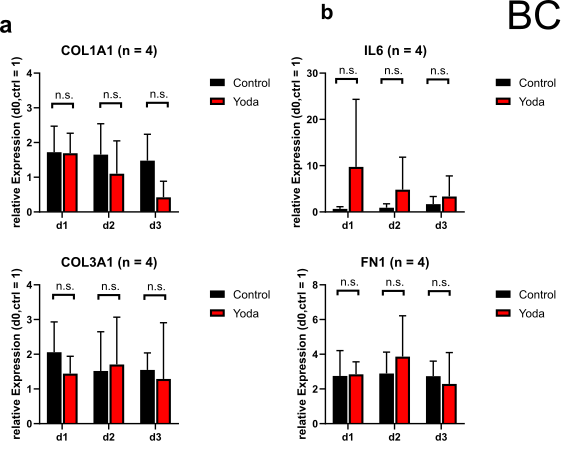
\includegraphics[scale = 0.6]{Collection.png}
    \caption{
    PCR Experiments where we saw some really cool stuff happening. 
    \textbf{a}: \colone output \textit{(n = 4)}
    \textbf{b}: Interleukin 6 out \textit{(n=23445)}
    All Experiments had n = 4. 
    }
    \label{fig:my_label}
\end{figure}

\subsection{WesternBlot}

\subsection{qRT-PCR}

\section{Excursion: Biostability of Yoda1}
\label{sec:biostability}